\section{Experimental Evaluation}

\TODO{
  \begin{itemize}
    \item CPU numbers for tree parallelization 
    \item Tahoe on T400
    \item Sensitivity analysis for schedules. But for what specifically? Models, batch sizes?
  \end{itemize}
}

\begin{figure}[htb]
  \centering
  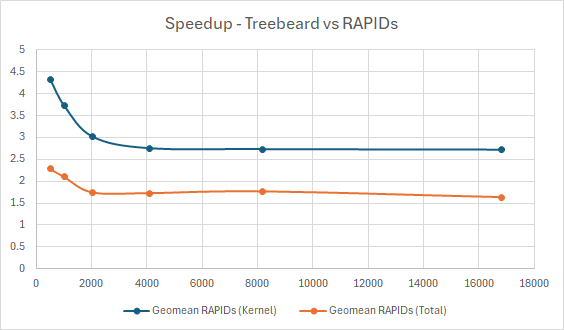
\includegraphics[width=\linewidth]{figures/TBvsRAPIDs_4060_Speedup.png}
  \caption{\Treebeard{} vs RAPIDs Speedup on NVIDIA RTX 4060.}
  \label{Fig:TBvsRAPIDs_4060_Speedup}
\end{figure}

\begin{figure}[htb]
  \centering
  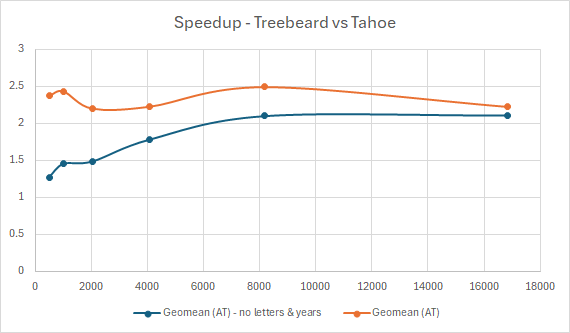
\includegraphics[width=\linewidth]{figures/TBvsTahoe_4060_KernelTimeSpeedup.png}
  \caption{\Treebeard{} vs Tahoe Kernel Time Speedup.}
  \label{Fig:TBvsTahoe_4060_KernelTimeSpeedup}
\end{figure}

\begin{figure}[htb]
  \centering
  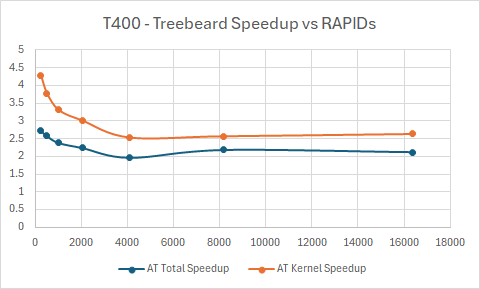
\includegraphics[width=\linewidth]{figures/TBvsRAPIDs_AllBatchSizes_T400.png}
  \caption{\Treebeard{} vs RAPIDs Speedup on T400.}
  \label{Fig:TBvsRAPIDs_AllBatchSizes_T400}
\end{figure}

\begin{figure}[htb]
  \centering
  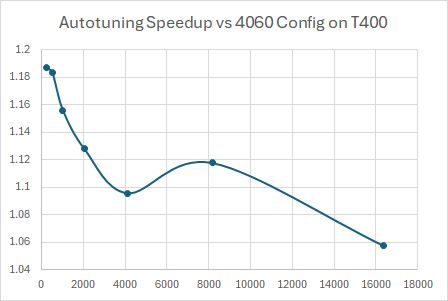
\includegraphics[width=\linewidth]{figures/AutotuningSpeedupvs4060Sched_T400.png}
  \caption{Autotuning heuristics speedup vs best 4060 schedule on T400.}
  \label{Fig:AutotuningSpeedupvs4060Sched_T400}
\end{figure}

\begin{figure}[htb]
  \centering
  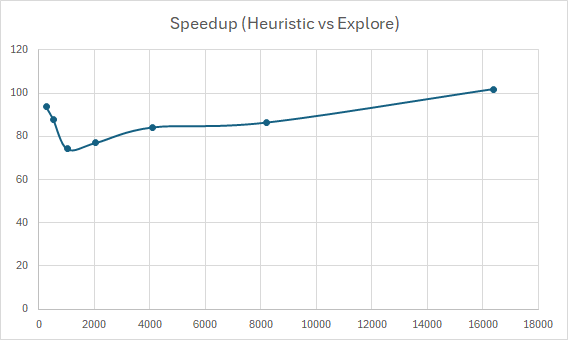
\includegraphics[width=\linewidth]{figures/HeuristicVsFullExplore_Speedup.png}
  \caption{Autotuning heuristic compile time speedup vs full schedule exploration.}
  \label{Fig:HeuristicVsFullExplore_Speedup}
\end{figure}

\begin{figure}[htb]
  \centering
  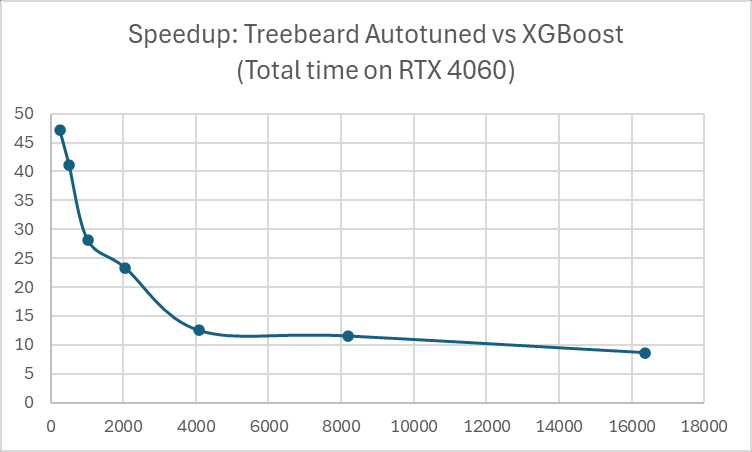
\includegraphics[width=\linewidth]{figures/TBvsXGB_TotalTime.png}
  \caption{\Treebeard{} vs XGBoost Speedup on RTX 4060.}
  \label{Fig:TBvsXGBoost_Speedup}
\end{figure}

\begin{figure}[htb]
  \centering
  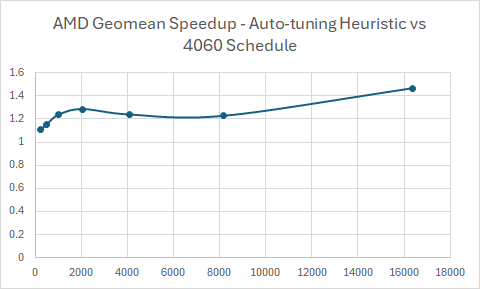
\includegraphics[width=\linewidth]{figures/AMD_MI210_ATHeuristicVs4060Sched_speedup.png}
  \caption{Autotuning heuristics speedup vs best 4060 schedule on MI210.}
  \label{Fig:AMD_MI210_ATHeuristicVs4060Sched_speedup}
\end{figure}

\begin{figure*}[ht]
  \centering
  \begin{subfigure}[b]{.3\textwidth}
    \subcaptionbox*{}{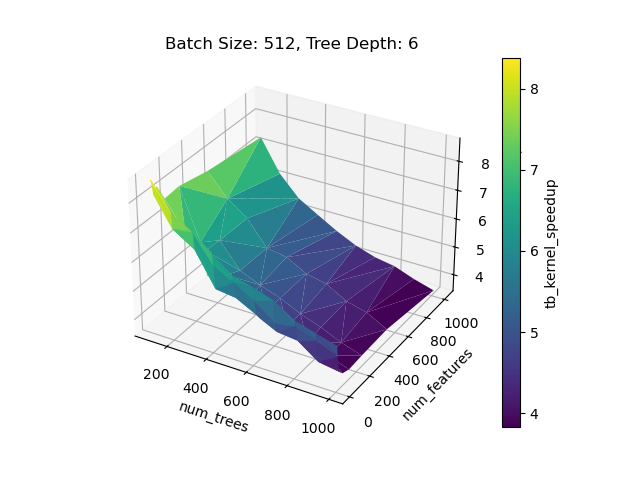
\includegraphics[width=\textwidth]{figures/RandomModels/kernel_speedup_b512_depth6.png}}
    \caption{Kernel Speedup for batch size 512, depth 6.}
  \end{subfigure}
  \hfill  % Add horizontal space between subfigures
  \begin{subfigure}[b]{.3\textwidth}
    \subcaptionbox*{}{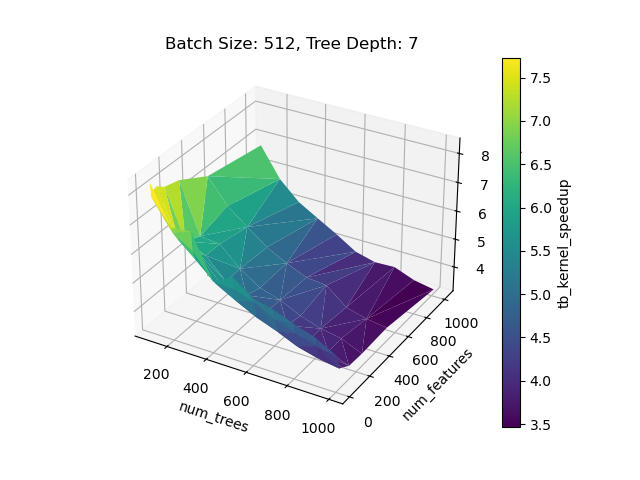
\includegraphics[width=\textwidth]{figures/RandomModels/kernel_speedup_b512_depth7.png}}
    \caption{Kernel Speedup for batch size 512, depth 7.}
  \end{subfigure}
  \hfill
  \begin{subfigure}[b]{.3\textwidth}
    \subcaptionbox*{}{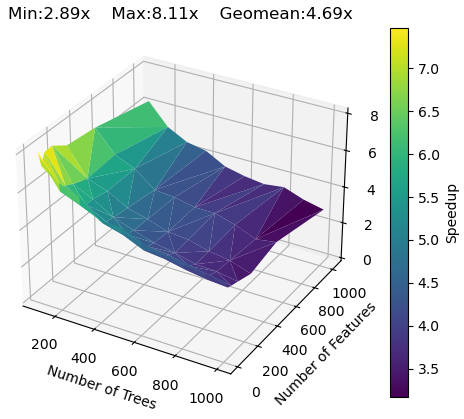
\includegraphics[width=\textwidth]{figures/RandomModels/kernel_speedup_b512_depth8.png}}
    \caption{Kernel Speedup for batch size 512, depth 8.}
  \end{subfigure}
  \\  % Line break for the second row
  \begin{subfigure}[b]{.3\textwidth}
    \subcaptionbox*{}{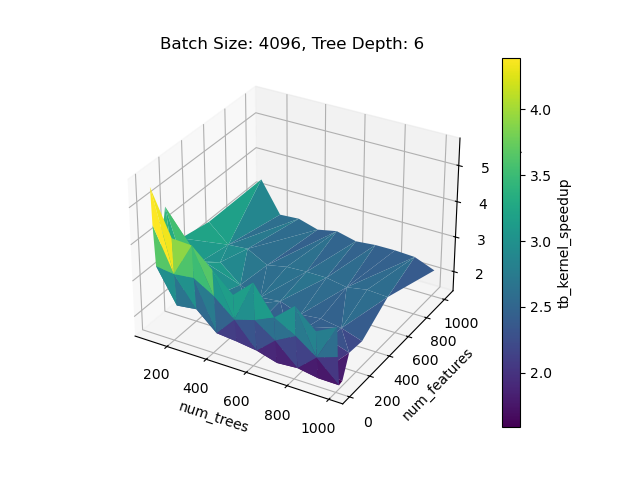
\includegraphics[width=\textwidth]{figures/RandomModels/kernel_speedup_b4096_depth6.png}}
    \caption{Kernel Speedup for batch size 4096, depth 6.}
  \end{subfigure}
  \hfill
  \begin{subfigure}[b]{.3\textwidth}
    \subcaptionbox*{}{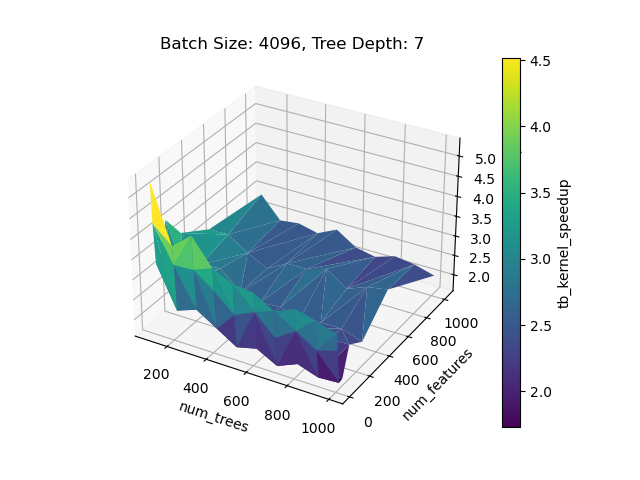
\includegraphics[width=\textwidth]{figures/RandomModels/kernel_speedup_b4096_depth7.png}}
    \caption{Kernel Speedup for batch size 4096, depth 7.}
  \end{subfigure}
  \hfill
  \begin{subfigure}[b]{.3\textwidth}
    \subcaptionbox*{}{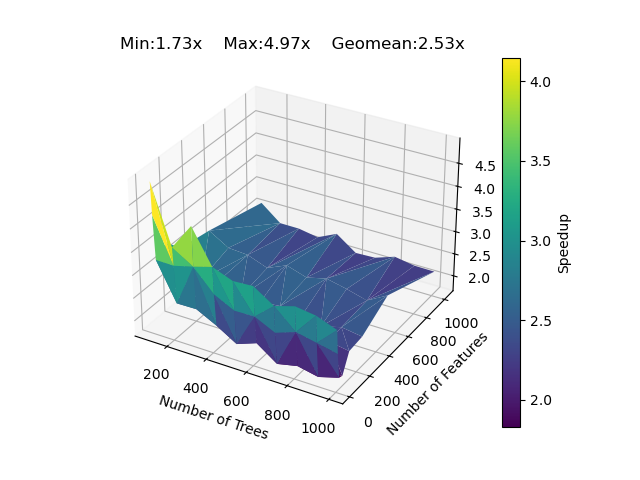
\includegraphics[width=\textwidth]{figures/RandomModels/kernel_speedup_b4096_depth8.png}}
    \caption{Kernel Speedup for batch size 4096, depth 8.}
  \end{subfigure}
\end{figure*}